\chapter{Previous Work}
\label{ch:2}

Section~\ref{sec:ch2-convetional-approaches} discusses the approaches that are conventionally used for evaluating storage subsystem designs. Section~\ref{ch2:summary} gives a summary of the related works.

\section {Conventional Approaches to Storage Subsystem Evaluation}
\label{sec:ch2-convetional-approaches}
\subsection {Simulation with I/O Traces}
\label{sec:ch2-simulation-with-IO-traces}

I/O traces are often used by designers to evaluate the performance of storage subsystem designs due to its simplicity. In this method, I/O requests are recorded on a real system and are then played back in a simulation environment to drive a standalone model of the storage subsystem of interest. Ganer and Patt~\cite{Ganger:1998} have investigated on issues associated with using standalone models for evaluating storage subsystem designs. In general, doing performance predictions using standalone storage subsystems models in isolation without considering the system-level behaviors can have the following two problems:

\begin{itemize}
	\item The workloads used for benchmarking are often not representative of the reality~--- The conventional methodology of generating benchmark workloads using I/O traces often ignores feedback effects between the storage subsystem and the workload source since the workloads are generated offline. Due to lack of system-level models, the I/O traces are often played back using either open or closed subsystem models. In the open subsystem models, the I/O requests are assumed to have predetermined arrival times. That is, the changes to the completion times of I/O requests do not have effect on the arrival of subsequent requests. In the closed subsystem models, subsequent I/O requests are assumed to be generated as soon as the previous requests have been completed. In both the open and closed subsystem models, the arrival pattern of the I/O requests is always the same as when they are recorded on the real system. However, in real systems, the completion time of each individual I/O requests can affect the pattern or arrival times of subsequent requests.

	\item Metrics used for measuring standalone storage subsystem performance are not always good indicators of the overall system performance~--- When standalone storage subsystem model is used for performance predictions, the metrics that can be used for performance measurement is limited. For example, it is not possible to measure the overall system performance using the elapsed time or throughput of the user tasks. Improvement to the metrics that can be measured using standalone models, such as the response time and throughput of I/O requests, cannot always be used as the indicator to the improvement of the overall system performance.
\end{itemize}

\subsection{Simulation with Abstract System-Level Models}

The problems associated with using standalone storage subsystem models can be alleviated by incorporating system-level models in the simulation. In this approach, system-level trace, instead of I/O-level trace, of a real system is recorded and played back in a simulation environment which also models the system-level behaviors of the real system.

Some of the system-level behaviors that can affect the performance of a storage subsystem as perceived by the user are discussed as follows. When trying to predict the performance of a storage subsystem, depending on the accuracy required by the prediction results, some or all of these system-level behaviors should be considered.

\begin{description}
	\item[I/O scheduling] In modern operating systems, I/O requests can be reordered or merged before actually being submitted to the underlying storage devices. This behavior is called I/O scheduling and is usually done for optimizing and balancing I/O request service times. The operation of the I/O scheduling algorithm is a dynamic behavior that depends on the state of the request queue and the arrival time and the order of the I/O requests. Benchmarking using pre-recorded I/O traces can overlook the impact of the I/O scheduling process on the storage subsystems.
	
	\item[File system mapping layer] Most real world applications are designed around file systems and do not access the underlying raw storage devices directly. Depending on the characteristics of the workload, using different file system mapping layers can have dramatic effects on the performance of the storage subsystems. Without modeling the behaviors of the file system mapping layer, it is sometimes not possible to accurately predict the performance of a storage subsystem design.
	
	\item[Dynamic data partitioning] A tiered storage subsystem have storage devices of different sizes and speeds; it will decide at run-time where to store the incoming I/O requests and will also move data among different tiers of storage devices. Benchmarking with prerecorded I/O traces cannot reproduce this kind of dynamic data partitioning behavior.
	
	\item[Caching] Caches are used at various layers in a system to improve performance; it can affect the actual workloads hitting the lower-level layers. For example, the I/O requests that actually hit the underlying storage devices are the ones that missed the upper layer caches. Depending on the target system’s cache configurations, I/O traces prerecorded with different system configurations might not be representative enough for testing the target system.
	
	\item[Virtual memory swapping] On operating systems that implement virtual memory, additional workloads could be imposed on the storage subsystem when memory swapping occurs. The overall performance of the storage subsystem can be affected by such additional workload.
	
	\item[Multi-tasking] In a multi-tasking system, the aggregated I/O workload submitted to the storage subsystem can be generated by concurrently running applications. Depending on the characteristics of the applications, for example, I/O-bound or CPU-bound, and the task scheduling algorithm, the aggregated I/O workload that will be generated cannot easily be simulated by I/O tracing techniques. 
\end{description}

It can be expected that modeling all of the aforementioned behaviors for simulation can take a great deal of work. Furthermore, even if one takes the effort to build and validate the abstract models for all of the essential system-level behaviors in a simulator, the chosen runtime parameters for each abstract model may not precisely simulate the real system. Depending on how subtle the design choices are, the differences can lead to inaccurate performance predictions and therefore wrong conclusions.

\subsection{Complete Machine Simulation}

\begin{figure}[htpb!]
	\centering
	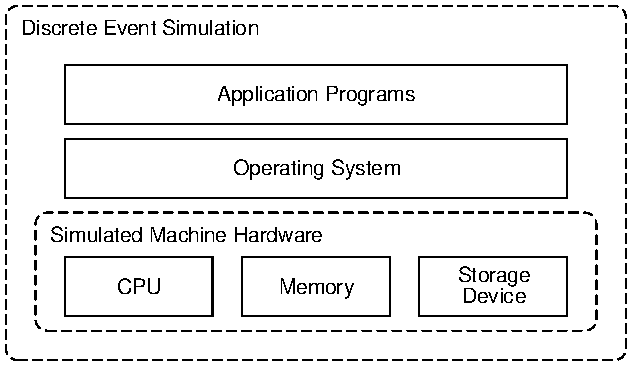
\includegraphics[width=0.65\textwidth]{figures/complete-machine-simulation.pdf}
	\caption{\label{fig:complete-machine-simulation}Complete machine simulation.}
\end{figure}

Complete machine simulation is one of the approaches which can allow the overall system performance to be evaluated with simulated storage devices that are not yet available. The concept of the complete machine simulation approach is illustrated in Figure~\ref{fig:complete-machine-simulation}. With complete machine simulation, a simulation model of the target machine hardware, including the storage device of interest, is first constructed.  The OS and application programs are then executed on the simulated machine hardware to study the overall system performance. An attractive attribute of the complete machine simulation approach is that it can be used for studying a wide range of system configurations – anything that can be modeled and simulated can be studied. Because the entire virtual machine model is simulated in the discrete-time domain, the performances and characteristics of the storage devices that can be simulated will not be limited by the performance of the simulation host. For example, it is possible to use a slower conventional hard disk drive for simulating large and faster solid-state drive (SSD) storage devices.

Unfortunately, one problem with the complete machine simulation approach is that the simulation speed of the complete machine model can be much slower than the speed of the native machine hardware. For example, in the SimOS environment~\cite{Rosenblum:1995}, simulation using the detailed CPU model can be 3 to 4 orders of magnitude slower than running the same workload on the native host.

Another problem with the complete machine simulation approach is the difficulties and efforts that are involved in constructing accurate complete machine models~\cite{Gibson:2000}, \cite{Gutierrez:2014}. Although there are simulators that are capable of running a sophisticated operating system, there are reports that show that their accuracy may differ from the real system when simulating memory-intensive tasks due to lack of exact memory subsystem models. Moreover, the internal design details of commercial SoCs might not be made publicly available by its manufactures~\cite{Eklov:2011}. In particular, accurate memory subsystem models (including the cache controller, the memory controller, and the DRAM models, etc.) are often not available for commercial embedded SoCs. For example, in~\cite{Butko:2012}, the differences in the real performance and simulated performance with the default models of the popular GEM5 simulator can be as large as 17.94\%.

%TODO: 
%---> Please note that ... Complete machine simulators that do not model accurate timings of the target hardware cannot be used for performance evaluations. For example, QEMU... copy some text from author's response here...

\subsection{Timing-Accurate Storage Device Emulation}
\label{sec:ch2-timing-accurate}

Timing-accurate storage device emulation is another approach that can be used for evaluating the overall system performance with simulated storage devices that are not yet available~\cite{Griffin:2002}. In timing-accurate storage device emulation, an emulated storage device is made available to the OS which is executing on the real machine hardware. The OS can interact with the emulated storage device similar to with a real storage device. The service timings of the emulated storage device are determined by a disk model which models the behavior of the target storage device. When an I/O request is submitted to the emulated storage device, the storage device emulator will need to carry out the following tasks:

\begin{enumerate}
\item Compute the response time of the I/O request by simulating the disk model.
\item Handle the actual data of the I/O request. If the I/O request is a write request, then the actual data is stored to the backing storage. Otherwise, the actual data is retrieved from the backing storage.
\item	Reply the I/O response to the OS at the corresponding service time as determined by the disk model.
\end{enumerate}

The conventional storage device emulators can conceptually be classified into two types of designs:
\begin{enumerate*}[label=(\roman*)]
	\item local virtual storage device emulation, and
	\item remote actual storage device emulation.
\end{enumerate*}
These two types of designs will be discussed in the follow subsections.

\subsubsection{Local Virtual Storage Device Emulation}

\begin{figure}[htpb!]
	\centering
	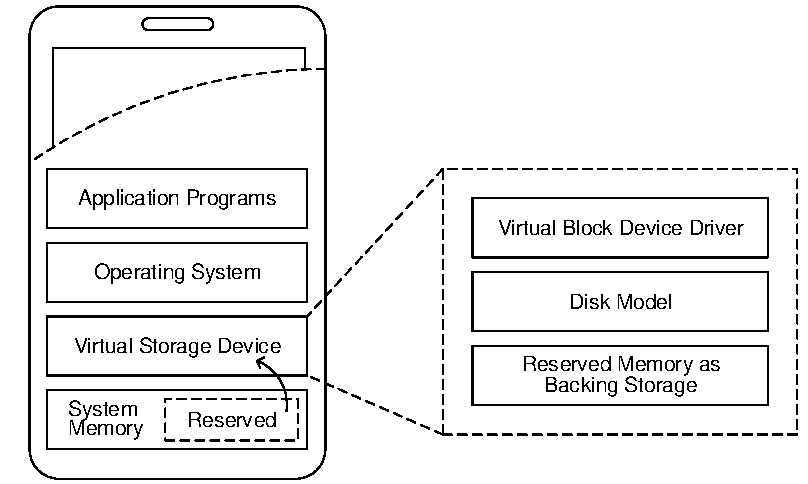
\includegraphics[width=0.8\textwidth]{figures/local-virtual-emulation.pdf}
	\caption{\label{fig:local-virtual-emulation}Local virtual storage device emulation.}
\end{figure}

An overview of the local virtual storage device emulation design (which will be referred to as the local emulation design for short for the rest of this dissertation) is illustrated in Figure~\ref{fig:local-virtual-emulation}. In the local emulation design, a virtual storage device is presented to the OS at the device driver level. The service timings of the emulated storage device are determined by a disk model which is simulated using the target system's CPU. A portion of the system memory is reserved and used as the backing storage for persisting the actual data of the emulated storage device.

While the local emulation design is convenient to implement, it has two notable limitations:

\begin{itemize}
	\item The size of the emulated storage device will be limited by the amount of the system memory that can be reserved for the backing storage. Embedded systems are usually configured with no more than a few gigabytes of memory, and therefore can greatly limit the size of the benchmark workload that can be used for evaluation. Furthermore, reducing the amount of the system memory that can be used by the OS will affect the original behavior of the system. If the remaining system memory is under a certain threshold, it can also prevent the proper execution of the desired benchmark workloads.
	
	\item Because the disk model is simulated using the target system's CPU, the emulator will consume CPU cycles of the target system and therefore will affect the original system behavior. More importantly, if the time that it takes to simulate the disk model exceeds the targeted service time of the corresponding I/O request, then the emulator will fail to emulate the intended behavior of the target storage device.
\end{itemize}

\subsubsection{Remote Actual Storage Device Emulation}

\begin{figure}[htpb!]
	\centering
	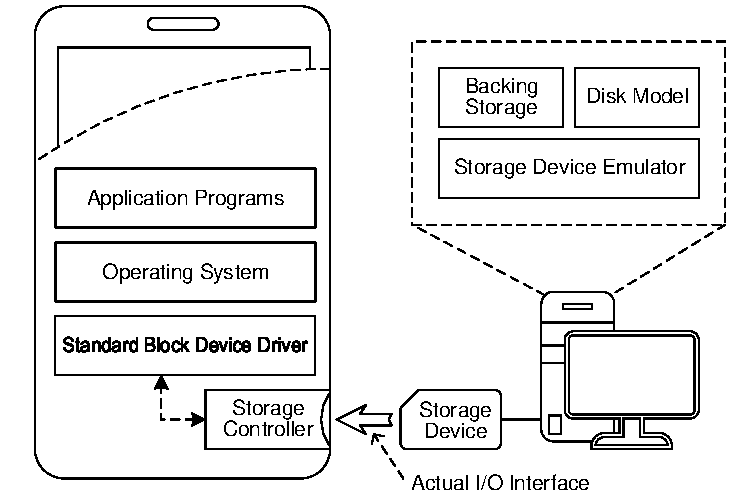
\includegraphics[width=0.75\textwidth]{figures/remote-actual-emulation.pdf}
	\caption{\label{fig:remote-actual-emulation}Remote actual storage device emulation.}
\end{figure}

An overview of the remote actual storage device emulation design (which will be referred to as the remote emulation design for short for the rest of this dissertation) is illustrated in Figure~\ref{fig:remote-actual-emulation}. In the remote emulation design, an actual storage device is emulated by the emulator software running on a separate computer and is presented to the OS at the actual I/O interface level. For example, if the target system has a Secure Digital (SD) card reader, then a storage device which is compatible to the SD standard can be emulated by the storage device emulator and inserted into the SD card reader of the target system.

Because the emulator software runs on a separate computer, the remote emulation design can overcome some of the problems faced by the local emulation design: Firstly, the size of the emulated storage device will not be limited by the size of the system memory available on the target system. It can be as large as the system memory or the backing storage available on the separate computer. Secondly, the CPU usage of the target system will not be affected by the emulator.

However, there are some limitations with the remote emulation design:

\begin{itemize}
	\item In both the local and remote emulation designs, the OS is running continuously in the real-time domain and the system time that the OS observes is progressing at the real-time speed. Therefore, in order to properly emulate the intended behavior of the target storage device, the conventional storage device emulators must be able to complete the processing of each I/O request in a timely fashion. The amount of time that is allowed for processing each I/O request is bounded by the service time of the particular I/O request. For example, if the computed service time of an I/O request is 1ms, then the total amount of time that can be used by the storage device emulator for simulating the disk model and accessing the backing storage cannot exceed 1ms. Otherwise, the performance of the emulated storage device will be slower than the intended target, which will lead to performance evaluation errors.
	
	\item The latency and bandwidth of the emulated storage device will be limited by the latency and bandwidth of the actual I/O interface. For example, the UHS-I bus interface defined by the SD standard has a maximum bus speed of 104MB/s, and therefore storage devices which are faster than 104MB/s cannot be emulated over the UHS-I interface. This kind of limitation can prevent the emulation of faster storage devices over existing I/O interfaces.
	
	\item The features that can be supported by the emulated storage device will be limited by the characteristics of the actual I/O interface. For example, because the SD interface protocol does not support more than one outstanding I/O requests concurrently, storage devices which have features such as Native Command Queuing (NCQ) cannot be emulated over the SD interface.
\end{itemize}

\section {Related Work}
\label{ch2:summary}

Proper evaluation of storage subsystems is not an easy task. Traeger et al.~\cite{Traeger:2008} have proposed a set of guidelines for proper storage subsystem performance evaluations.
% TODO: Summarize the guide lines here.
Using the guidelines as the evaluation criteria, they have surveyed 415 file system and storage benchmarks from a selection of conference papers between the year 1999 and 2007. The selected benchmarks are all conducted on real machine environments. They have found that most benchmarks are flawed and could give the readers wrong impressions on the real performance of the storage subsystems under test and even lead to incorrect design conclusions. From the guidelines, it can be clearly seen that it is important that the system-level behaviors are taken into account when performing storage subsystem evaluation.

In the work of Ganger and Patt~\cite{Ganger:1998}, they have constructed abstract system-level model that contains necessary host system component modules with appropriate details for generating workloads for benchmarking storage subsystems. System-level traces, instead of I/O traces, are recorded on real system and played back using the abstract system-level model for generating workloads to drive the storage subsystem module.

Instead of using purely abstract models for system-level simulation, Thekkath~\cite{Thekkath:1994} incorporated real file system code into the simulation system. In his approach, I/O traces are gathered on real systems and are used to drive the real file system code in the simulation process for generating I/O requests.

An alternative to using abstract system-level models for performing storage subsystem evaluations is to use complete machine simulation. The SimOS environment~\cite{Rosenblum:1995}, \cite{Witchel:1996}, \cite{Rosenblum:1997} is a complete machine simulator which can simulate the hardware of an SGI machine in enough detail to run the Irix OS. SimOS supports switching among a number of hardware component models which are different in terms of modeling detail and accuracy. The less detailed models can run faster and can be used to boot and position the system into a state at which interesting workloads will begin. The simulation can then switch to use a more accurate model for detailed profiling. Griffin et al.~\cite{Griffin:2000} has integrated a MEMS-based storage device simulator into the SimOS environment for studying the performance and characteristics of MEMS-based storage devices. Although complete machine simulation does allow the actual OS and real applications to be run on the simulated machine hardware, it can run much slower than the real system. Furthermore, building and maintaining accurate complete machine simulation models could take substantial amount effort.

Timing-accurate storage emulation has been explored in detail by Griffin et al. \cite{Griffin:2002}. Memulator allows researchers to explore with nonexistent storage devices and take end-to-end measurements in full-system contexts. Memulator can use either the memory of the local machine or a networked machine as the backing storage for the emulated disk. Their work gives support that storage device emulation is an effective method for studying the overall system performance with simulated virtual storage devices. In their remote emulation setup, the emulator is executed on a standalone computer and connected to the target system over the SCSI interface. The DiskSim simulator~\cite{Bucy:2008} is used for simulating the service times of the Seagate Cheetah X15 hard disk drive. Experimental results show that the benchmark results measured with the emulated storage device are close to the results measured with the real storage device.

In the work of Maghraoui et al.~\cite{ElMaghraoui:2010}, a local emulation type storage device emulator is developed to emulate flash based SSD for the AIX OS. The emulator is implemented as a dynamic loadable kernel module and appears to the OS as a disk device. A chunk of system memory is pined for use as the backing storage, and high resolution nanosecond granularity timers are used for simulating the delays of the I/O operations. Lee et al.~\cite{Lee:2012} have proposed another local emulation type SSD emulator. The target platform is the Linux OS and it uses a user mode SSD simulation engine for calculating the latencies for the I/O requests. The backing storage used can be either the system memory or some other external DRAM-based storage devices.

David~\cite{Agrawal:2012} is another local emulation type storage device emulator which is mostly concerned about the required backing storage size for emulating large storage devices. The main idea of David is to reduce the data that needs to be saved to the backing storage so that larger storage devices can be emulated using less storage space. The key idea is that for certain types of benchmark workloads, the actual content in the file system files can be omitted and only file system metadata needs to be persisted onto the backing storage. By not persisting the actual content in the files, David is able to reduce the storage size requirements by orders of magnitude. David has been demonstrated to work with the ext3 and the btrfs~\cite{wiki:btrfs} file systems, and in theory, it can be extended to work with other types of file systems.

VSSIM~\cite{Yoo:2013} is a virtual machine (VM) based SSD simulator which makes emulated SSD devices available to the VM. The emulated SSD device appears to the VM as a storage device connected to the IDE interface. VSSIM runs in real-time and allows the user to measure both the host performance and the SSD behavior under various design choices. The design of VSSIM can conceptually be classified as similar to the remote emulation design. The difference is that the target machine that the emulated storage device is ``connected'' to is a VM, and therefore VSSIM does not need to emulate the actual electrical signals of the IDE interface.

Finally, Canon et al.~\cite{Canon:1980} extended the standard virtual machine (VM) environment to include virtual time emulation. In contrast to the conventional VM environment, in which the real time of day (RTOD) clock is observed by the VM, the modified VM environment makes the VM to observe a virtual time of day (VTOD) clock. The VTOD clock progresses as program instructions are executed on the virtual CPU of the VM. In the modified VM environment, the system performance is evaluated against the VTOD clock. The VM environment proposed by Canon et al. can be viewed as analogous to the SimOS environment configured with the direct execution model, in which the machine instructions are executed on the native CPU whenever possible and that the internal architecture of the CPU is not modeled.
